\documentclass{article} % For LaTeX2e
\usepackage{nips14submit_e,times}
\usepackage{amsmath}
\usepackage{amsthm}
\usepackage{amssymb}
\usepackage{mathtools}
\usepackage{hyperref}
\usepackage{url}
\usepackage{algorithm}
\usepackage[noend]{algpseudocode}
%\documentstyle[nips14submit_09,times,art10]{article} % For LaTeX 2.09

\usepackage{mathrsfs}
\usepackage{graphicx}
\usepackage{caption}
\usepackage{subcaption}

\def\eQb#1\eQe{\begin{eqnarray*}#1\end{eqnarray*}}
\def\eQnb#1\eQne{\begin{eqnarray}#1\end{eqnarray}}
\providecommand{\e}[1]{\ensuremath{\times 10^{#1}}}
\providecommand{\pb}[0]{\pagebreak}


\def\Qb#1\Qe{\begin{question}#1\end{question}}
\def\Sb#1\Se{\begin{solution}#1\end{solution}}

\newenvironment{claim}[1]{\par\noindent\underline{Claim:}\space#1}{}
\newtheoremstyle{quest}{\topsep}{\topsep}{}{}{\bfseries}{}{ }{\thmname{#1}\thmnote{ #3}.}
\theoremstyle{quest}
\newtheorem*{definition}{Definition}
\newtheorem*{theorem}{Theorem}
\newtheorem*{lemma}{Lemma}
\newtheorem*{question}{Question}
\newtheorem*{preposition}{Preposition}
\newtheorem*{exercise}{Exercise}
\newtheorem*{challengeproblem}{Challenge Problem}
\newtheorem*{solution}{Solution}
\newtheorem*{remark}{Remark}
\usepackage{verbatimbox}
\usepackage{listings}

\title{Real Variables: \\
Problem Set IX}


\author{
Youngduck Choi \\
Courant Institute of Mathematical Sciences \\
New York University \\
\texttt{yc1104@nyu.edu} \\
}


% The \author macro works with any number of authors. There are two commands
% used to separate the names and addresses of multiple authors: \And and \AND.
%
% Using \And between authors leaves it to \LaTeX{} to determine where to break
% the lines. Using \AND forces a linebreak at that point. So, if \LaTeX{}
% puts 3 of 4 authors names on the first line, and the last on the second
% line, try using \AND instead of \And before the third author name.

\newcommand{\fix}{\marginpar{FIX}}
\newcommand{\new}{\marginpar{NEW}}

\nipsfinalcopy % Uncomment for camera-ready version

\begin{document}


\maketitle

\begin{abstract}
This work contains solutions to the problem set 
IX of Real Variables 2015 at NYU.
\end{abstract}

\section{Solutions}

\begin{question}[1. Royden 12-5]
\hfill
\begin{figure}[h!]
  \centering
    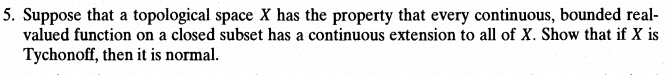
\includegraphics[width=1\textwidth]{12-5.png}
\end{figure}
\end{question}
\begin{solution}
Assume that $X$ is Tychonoff, and let $A$ and $B$ 
be non-empty disjoint closed subsets of 
$X$. Let $g:A \cup B \to \mathbb{R}$ such that  
such that $g(A) = a$ and $g(B) = b$. Observe that $g$ is a real-valued
function, that is continuous, bounded, on a closed subset of $X$. 
Therefore, by the given, there exists a continuous extension to 
all of $X$, which we denote as $g':X \to \mathbb{R}$. Observe that
as $(a-\dfrac{a+b}{2},\dfrac{a+b}{2})$ is open in $\mathbb{R}$, 
by the continuity of $g'$
we have $g'^{-1}((a-\dfrac{a+b}{2},\dfrac{a+b}{2}))$ is open in $X$, 
which contains 
$A$. Likewise, $g'^{-1}((\dfrac{a+b}{2},b+\dfrac{a+b}{2}))$ 
is open in $X$, which contains
$B$. Notice that as $g'$ is a function those two open sets are disjoint.
Therefore, we have shown that $A$ and $B$ have neighborhoods that are 
disjoint. Since $X$ is Tychonoff as well, $X$ is normal. 
\hfill $\qed$
\end{solution}

\bigskip

\begin{question}[2. Royden 12-6]
\hfill
\begin{figure}[h!]
  \centering
    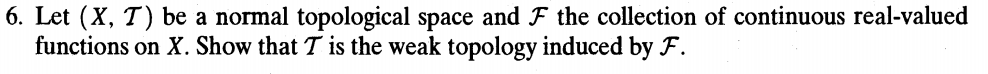
\includegraphics[width=1\textwidth]{12-6}
\end{figure}
\end{question}
\begin{solution}
Let $x \in X$. Consider a neighborhood $U_x \in \mathscr{T}$. It follows
that $X \setminus U_x$ is closed in $\mathscr{T}$. As normal topological 
spaces are Tychnoff, and single points are closed in Tychnoff spaces, we have
$\{ x\}$ is closed in $\mathscr{T}$. Then, by the Urysohn's lemma, 
we have a continuous real-valued function
$f:X \to [a,b]$ such that $f(\{x\} ) = a$ and
$f(X\setminus U_x ) = b$. Note that $f \in \mathscr{F}$.
Then, for a fixed $\epsilon$ 
such that $b -a > \epsilon > 0$,
as $(a-\epsilon ,a+\epsilon)$ is an open set in $\mathbb{R}$,
we have $f^{-1}((a-\epsilon,a+\epsilon))$
 is a basic open set of the weak-topology,
as $f$ is continuous and it's a finite intersection of the inverse
image of an open set.
Observe that as $f(X \setminus U_x) = b$, we have  
$f^{-1}((a-\epsilon,a+\epsilon)) \cap X \setminus  U_x = \emptyset$. Hence
$f^{-1}((a-\epsilon,a+\epsilon)) \subseteq U_x$. 
Therefore, we have found a basic 
open set of $x$ in the weak topology contained in $U_x$. Hence, we have that
the basis of weak-topology is a collection of open sets in $\mathscr{T}$,
such that for each $x$ and each neighborhood of $x$, $U_x$, there is an
element of the basis of weak-topology, that is contained in $U_x$. Therefore,
the basis of weak-topology, induced by $\mathscr{F}$
 is a also basis of the strong topology. Hence, in this case, the strong
topology $\mathscr{T}$ is the  
weak-topology induced by $\mathscr{F}$. 
\hfill $\qed$


\end{solution}

\bigskip

\begin{question}[3. Royden 12-27]
\hfill
\begin{figure}[h!]
  \centering
    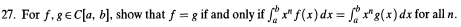
\includegraphics[width=1\textwidth]{12-37}
\end{figure}
\end{question}
\begin{solution}
Assume that $f = g$. Fix $n$. 
As $f,g \in C[a,b]$, $x^n \in C[a,b]$.
 and multiplication of continuous
function is continuous, we have that $x^n f$ and $x^ng$ are continuous.
As continuous functions on compact domain is integrable, by 
the linearity of integration, we have
\eQb
\int_{a}^{b} x^nf(x)dx - \int_{a}^{b} x^n g(x) dx 
&=& \int_{a}^{b} x^n(f-g)(x) dx \\.
\eQe
As $f = g$, $f-g(x) = 0$ for all $x \in [a,b]$. It follows that
\eQb
\int_{a}^{b} x^nf(x)dx - \int_{a}^{b} x^n g(x) dx &=& 0, 
\eQe
from which we obtain
\eQb
\int_{a}^{b} x^nf(x)dx &=& \int_{a}^{b} x^n g(x) dx. 
\eQe
Since $n$ was arbitrary, we have that the above equality holds for all $n$.
Conversely, assume that 
$ \int_{a}^{b} x^nf(x)dx = \int_{a}^{b} x^n g(x) dx$ for all $n$. By 
appealing to the linearity of integration, we see that
\eQb
\int_{a}^{b} p(f-g)(x) dx = 0, 
\eQe 
for any polynomial $p$ defined on $[a,b]$. We claim that
\eQb
\int_{a}^{b} (f-g)^2(x) dx = 0, 
\eQe 
which will imply that $f = g$ almost everywhere immediately.  
By Weiestrass Approximation theorem, we can choose a sequence of polynomials
$p_n$ such that
\eQb
|p_n - (f-g)| < \dfrac{1}{n}. 
\eQe
It follows that $\{ p_n (f-g) \}$ converges to $(f-g)^2$ pointwise 
everywhere on $[a,b]$. As $|p_n - (f-g) | < 1$ for all $n$ on $[a,b]$. 
As $f-g$ is a continuous function defined on a compact subset of $\mathbb{R}$,
by the extreme value theorem, there exists $M > 0$ such that 
$|f-g| < M$ on $[a,b]$. It follows that $g(x) = M(M+1)$ on $[a,b]$ is 
integrable and dominates $\{ p_n (f-g)\}$. Hence, by the Dominated
Convergence theorem, we have
\eQb
\int_{a}^{b} (f-g)^2(x) dx &=& \lim_{n \to \infty}
\int_{a}^{b} p_n(f-g)(x) dx.
\eQe 
Since $\int_{a}^{b} p_n(f-g)(x) dx = 0$ for all $n$, it follows that
\eQb
\int_{a}^{b} (f-g)^2(x) dx &=& 0.
\eQe
Hence, we conclude that $ f = g$ almost everywehre. As $f,g \in C[0,1]$,
and $f=g$ almost everywhere, it follows that $f = g$ everywhere.
\hfill $\qed$


 
\end{solution}

\newpage

\begin{question}[4. Royden 12-35]
\hfill
\begin{figure}[h!]
  \centering
    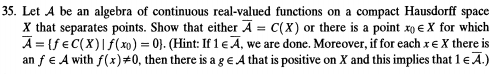
\includegraphics[width=1\textwidth]{12-35}
\end{figure}
\end{question}
\begin{solution}
Consider
\eQb
\mathscr{S} &=& \{ f^{-1}(O) \> | \> f \text{ is continuous, and } O
\text{ is open in} \mathbb{R} \}.
\eQe

\end{solution}

\newpage

\begin{question}[5. Royden 13-8]
\hfill
\begin{figure}[h!]
  \centering
    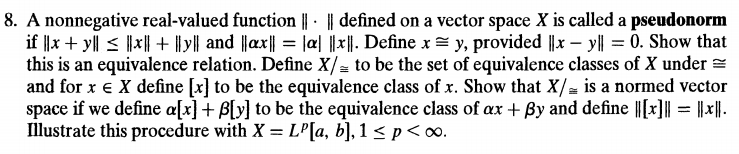
\includegraphics[width=1\textwidth]{13-8}
\end{figure}
\end{question}
\begin{solution}
We show that the pseudo-norm relation is 
reflexive, symmetric, and transitive.

\smallskip

Let $x \in X$. It follows that
\eQb
\lVert x - x \rVert = \lVert \theta \rVert,
\eQe
where $\theta$ is the identity element of the linear space $X$. By definition of linear space,
we have $\alpha \cdot \theta = \theta$ for all $\alpha$. Hence, for some $\alpha > 1$, we have 
\eQb
\lVert \theta \rVert &=& \lVert \alpha \cdot \theta \rVert \\
&=& | \alpha | \lVert \theta \rVert. \\
\eQe
As $|a| > 0$, we have  $|\theta | = 0$. Consequently, $\lVert x - x \rVert = 0$. It follows that
for all $x \in X$, $x \equiv x$. The relation is reflexive. 

\smallskip

Let $x,y \in X$ and $x \equiv y$. Observe that
\eQb
\lVert x - y \rVert &=& \lVert -1\cdot (y - x) \rVert \\
&=& |-1|\lVert y - x \rVert \\
&=& \lVert y - x \rVert. \\
\eQe
As $x \equiv y$, which gives $\lVert x - y \rVert = 0$, it follows that
$\lVert y - x \rVert = 0$ and $y \equiv x$. Hence, the relation is symmetric. 

\smallskip

Let $x,y,z \in X$ and $x \equiv y$ and $y \equiv z$. By triangle inequality, it follows that
\eQb
\lVert y - z \rVert &=& \lVert (x-y) + (y-z) \rVert \\
&\leq& \lVert x -y \rVert + \lVert y - z \rVert = 0 + 0 = 0.
\eQe
Hence, $\lVert y - z\rVert = 0$, and it follows that $x \equiv z$. 
Hence, the relation is symmetric. It follows that the pseudo-norm relation
is an equivalence relation on the linear space $X$.

\hfill $\qed$ 

\smallskip 

We show that $X\/_{\equiv}$ is a normed vector space. Firstly, we check that the defined norm
is well defined. Let $x,y \in X$, such that $x \equiv y$. It follows that $\lVert x - y \rVert = 0$.
Hence, $\lVert x \rVert = \lVert y \rVert$, and it follows that $\lVert [x] \rVert = \lVert [y] \rVert$.
The norm is well-defined. 



\end{solution}

\bigskip

\begin{question}[6. Royden 13-33]
\hfill
\begin{figure}[h!]
  \centering
    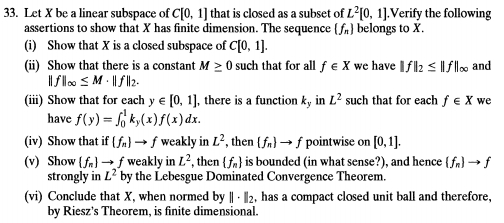
\includegraphics[width=1\textwidth]{13-33}
\end{figure}
\end{question}
\begin{solution}
Consider
\eQb
\mathscr{S} &=& \{ f^{-1}(O) \> | \> f \text{ is continuous, and } O
\text{ is open in} \mathbb{R} \}.
\eQe

\end{solution}

\end{document}
